\section{Beam Source}

\subsection{Physical structure}

\subsubsection{Cell assembly}

The cell assembly is rigidly attached to the tapped holes on the cold head of
the PT815 pulse tube cryocooler using six equally spaced (BCD = 3.40")
M$5\times0.8$ brass screws. During design, I was careful not to exceed 5~kg
suspended from the cold head as recommended by the pulse tube manufacturer; the
estimated cell assembly weight is approx.\ 3~kg.

\paragraph{Neon supply}

\subsubsection{Heat shields}

\paragraph{4~K shield}

The 4~K shield is a box made out of six 1/4"-thick oxygen-free high
conductivity copper (OFHC) plates with cutouts for the pulse tube head to reach
the cell, as well as for the molecular and laser beams to enter or exit the
shield. The box is suspended from the top plate of the 40~K shield using
stainless 1/4-20 threaded rods, secured with brass nuts.

\paragraph{40~K shield}

The 40~K shield is also a box, however the assembly consists of two sets of
parts: the internal structure (visible in Fig.~\ref{40K_internal}, left) and the
cover plates (Fig.~\ref{40K_internal}, right).

\begin{figure}
    \centering
    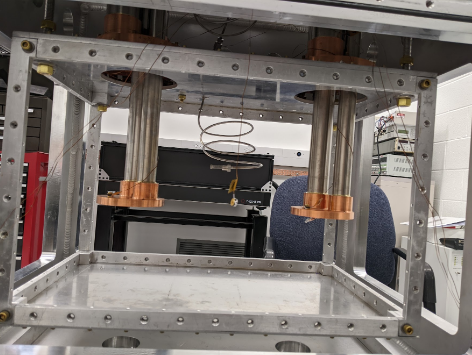
\includegraphics[height=.35\textwidth]{figs/todo/40K_internal.png}
    \hfill
    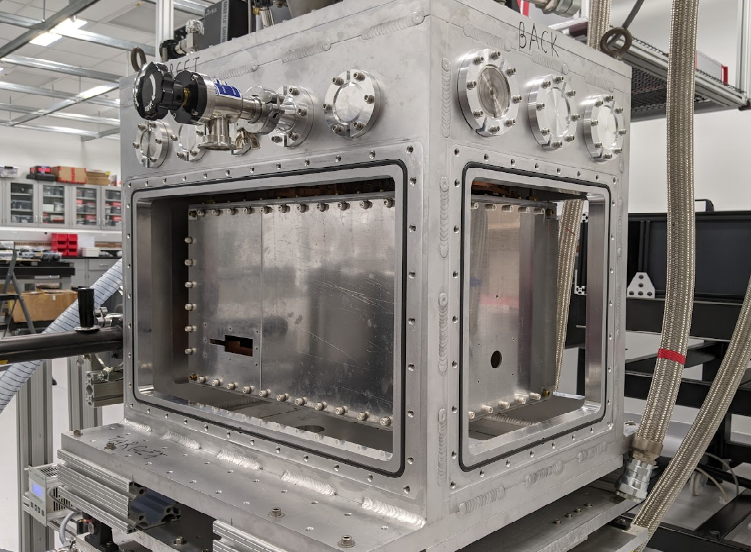
\includegraphics[height=.35\textwidth]{figs/todo/40K_closed.png}
    \caption[40~K shield.]{40~K shield. \part{Left} Internal structure of the
    40~K shield. \part{Right} Vacuum chamber with cover plates removed, showing
    the closed 40~K shield inside.}
    \label{40K_internal}
\end{figure}

Due to the large size of the 40~K shield, it is made out of 1100-alloy aluminum
despite roughly an order of magnitude worse thermal conductivity compared to
OFHC copper \cite[Fig.~6.13]{ekin2006experimental}; the conductivity is not
crucial. Originally, the plates were 1/4" thick, but were later changed for
0.09" thick plates (waterjet from stock, McMaster p.n.\ 88685K94) to speed up
the amount of time needed to reach cryogenic temperatures.

The 40~K box is suspended from the top plate of the vacuum chamber using 3/8"
stainless threaded rods, secured with brass nuts and Belleville washers. We have
considered using a thin-walled threaded tube for these standoffs to decrease
thermal conductivity, however the solid threaded rods in practice do not pose
any problems and the heat shield can easily reach the desired temperature.

\paragraph{Flexible heat links}

Due to different thermal expansion coefficients of different metals, the parts
of the beam source will end up at slightly different relative positions when
operating at the cryogenic temperature. To prevent the potential stress on the
delicate pulse tubes, we attach them with flexible heat links. The heat links
are the only thing attached to the `warm stage' of the pulse tubes and they are
well below the weight limit of 10~kg per pulse tube warm stage.

We have two pulse tubes in our beam source. The lower-temperature PT415 is
connected with a flexible link to the 4~K shield, while PT815 attaches directly
to the cell assembly (hidden within the 4~K shield). The 40~K `warm' stages of
both pulse tubes are connected with flexible links to the top plate of the 40~K
shield (Fig.~\ref{40K_heatlinks}).

\begin{figure}
    \centering
    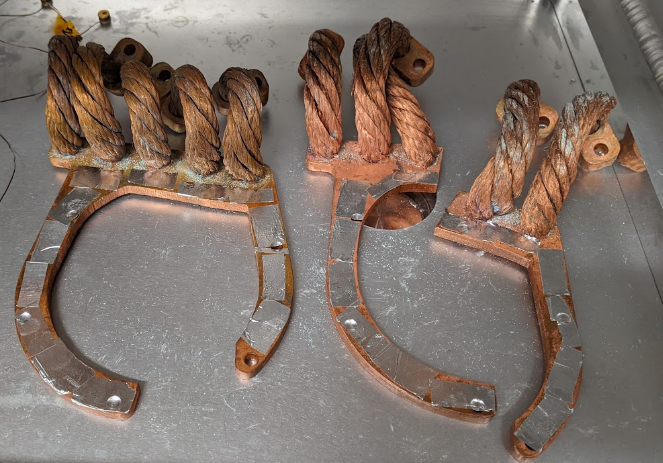
\includegraphics[height=.34\textwidth]{figs/todo/heatlink.png}
    \hfill
    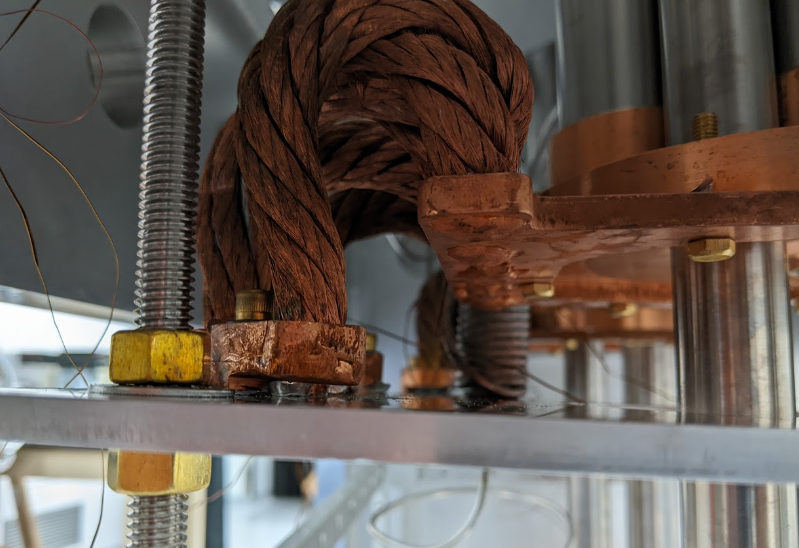
\includegraphics[height=.34\textwidth]{figs/todo/heatlink_attached.png}
    \caption[Flexible heat links for the 40~K shield.]{Flexible heat links for
    the 40~K shield. \part{Left} Before attaching to the cryostat. One of the
    links is cut into half for ease of assembly. \part{Right} Screwed into the
    40~K top plate as well as the `warm stage' of the pulse tubes.}
    \label{40K_heatlinks}
\end{figure}

The flat end pieces of the heat links were cut with a waterjet from 1/4" thick
101-alloy copper plates (McMaster p.n.\ 3350K215), while the smaller ends were
cut out of a 1/2" plate (McMaster p.n.\ 3350K223). After machining, I cleaned
the parts in 2\%\ Citranox solution and deionized water (20 minutes of
ultrasonic cleaning in each of the two liquids).

Each heat link piece includes five stranded C10100-alloy copper cables (Cooner
Wire, p.n.\ NER 7710836 B-OFE) welded by the Harvard machine shop (courtesy of
Benjamin Augenbraun from John Doyle's group).  Due to the high thermal
conductivity of the copper cables, brazing is impossible as the braze would wick
up the braid, solidify there, and render the heat link inflexible. The copper
braid could also be clamped, but welded is a more reliable way to achieve a high
thermal conductivity. After the welding, I cleaned the heat links by submerging
them in an ultrasonic bath of a Citranox solution for three hours at 80\degC,
then changed the water (by then completely green) for another hour of Citranox,
rinse in tap water, ultrasonically clean in tap water, and in acetone, and in DI
water.

\subsubsection{Vacuum chamber}

The vacuum chamber has been fabricated by Atlas Technologies out of 6061-alloy
aluminum. The chamber consists of a welded box and a set of six cover plates
(Fig.~\ref{beam_source_vacuum}). For ease of mounting the chamber onto a stand,
as well as attaching various components to the chamber (e.g., optics), the
bottom of the welded part has `wings' that extend outwards perpendicular to the
beam direction, with two rows of 1/4-20 tapped holes, spaced by 2", on each
wing. The entire beam source can be lifted using the four 3/8-16 eye bolts that
pass through the top cover plate (Fig.~\ref{top_plate}) into four corresponding
tapped holes inside the main chamber body.

\begin{figure}
    \centering
    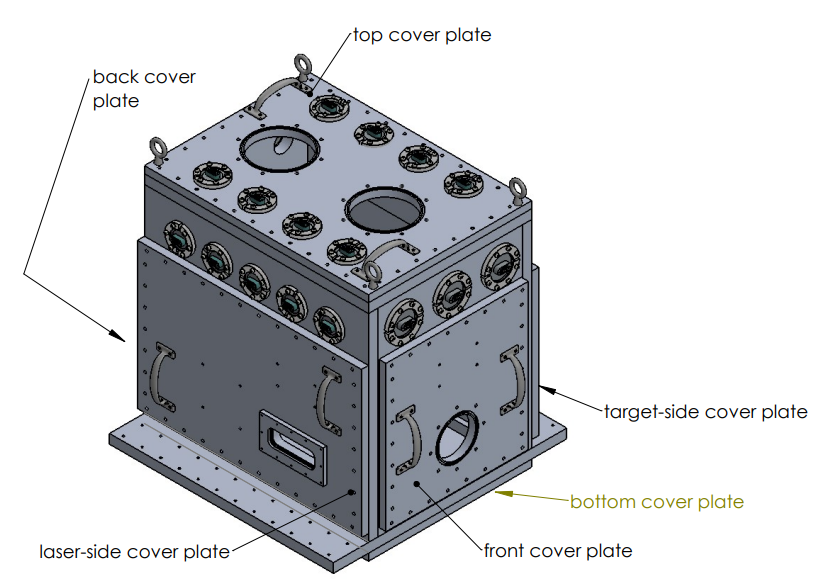
\includegraphics[width=\textwidth]{figs/todo/beam_source_vacuum.png}
    \caption{Beam source vacuum chamber.}
    \label{beam_source_vacuum}
\end{figure}

\begin{figure}
    \centering
    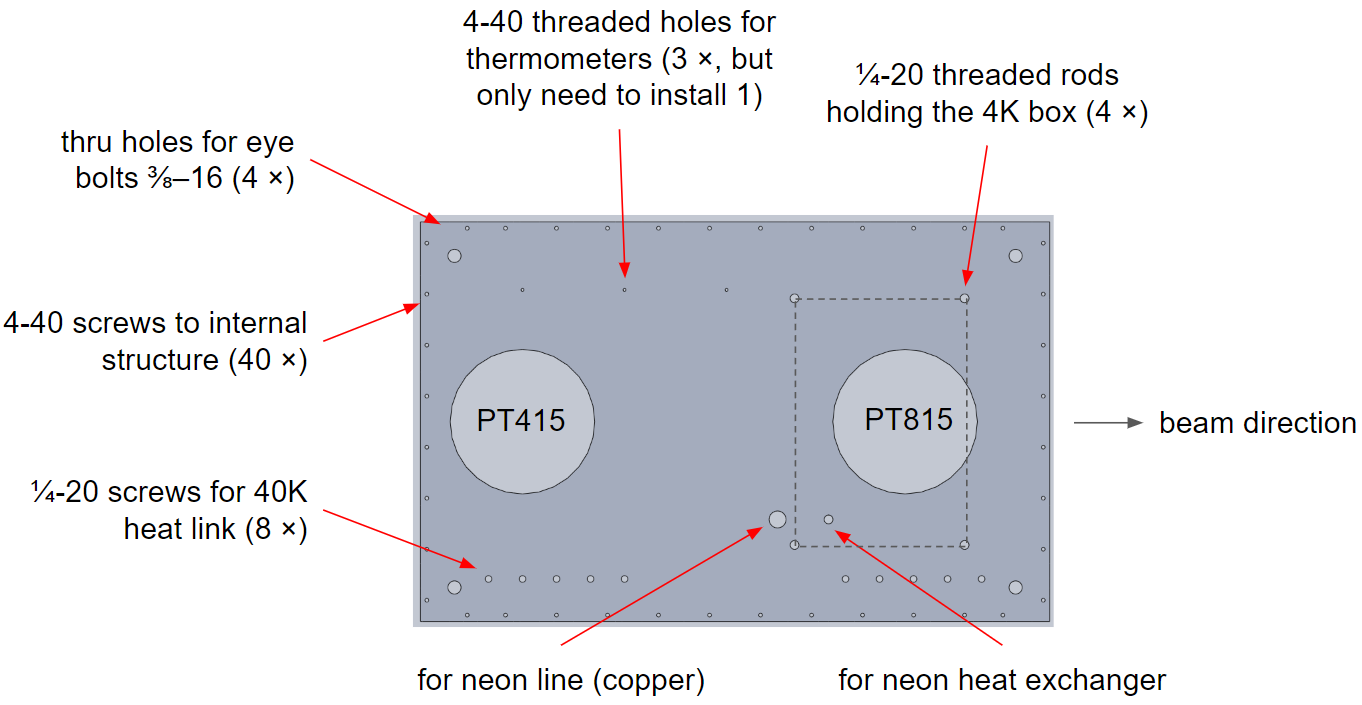
\includegraphics[width=\textwidth]{figs/todo/top_plate.png}
    \caption{Beam source vacuum chamber top plate.}
    \label{top_plate}
\end{figure}

The cover plates are sealed onto the welded structure using round O-rings (1/4"
fractional diameter, 0.275" actual cross-section diameter) seated into
dovetailed grooves.

\subsubsection{Electronic connections}

There are two groups of electronic connections to the beam source, namely
heaters and temperature sensors. The heaters are all connected to a single DB-9
feedthrough, as follows:\\

\begin{tabular}{rl}
1--2 & two 10~$\Omega$ cell bottom heaters connected in series (CTC100 output
    1)\\
3--4 & four 50~$\Omega$ 16K cell top plate heaters (CTC100 output 2)\\
6--7 & disconnected (formerly snorkels)\\
8--9 & five 4~K shield 10~$\Omega$ heaters, in series
\end{tabular}\\

The original design used polyimide film insulated flexible heaters, namely a
$3"\times3"$ square heater between the cell top plate and the plate attached to
the pulse tube, and a 2" round heater clamped on the bottom side of the cell.
During first use, these heaters overheated and burned out, presumably because of
insufficiently homogeneous thermal contact. These have been replaced by
standard high-power (i.e., 50--250~W) resistors in the TO-220 package. Since all
these heaters are cooled to cryogenic temperatures, we have experienced no
vacuum issues due to their outgassing despite not following any special cleaning
or testing precautions.

The 12 thermometers are read out via the 4-wire technique and are thus spread
between two DB-25 and two DB-9 feedthroughs. The ($I-,V-,V+,I+$) pin numbers for
each of the four connectors are as follows:\\

\begin{tabular}{rl}
   DB-25 & 1: back snorkel ($15,16,4,3$), 2: 4~K shield top plate ($18,19,7,6$) \\
         & 3: 40~K shield top plate ($21,22,9,10$), 4: 4~K PT ($24,25,13,12$) \\
   DB-25 & 5: cell top plate ($15,16,4,3$), 6: 4~K shield bottom plate ($18,19,7,6$) \\
         & 7: 40~K shield bottom plate ($21,22,9,10$), 8: 16~K PT ($24,25,13,12$) \\
   DB-9  & 9: input nozzle ($1,2,3,4$), 10: cell top plate target side ($6,7,8,9$) \\
   DB-9  & 11: 4~K PT warm stage ($1,2,3,4$), 12: 16~K PT warm stage ($6,7,8,9$)
\end{tabular}\\

All thermometers are silicon-diode sensors (Lake Shore Cryotronics, Inc., p.n.\
DT-670, CU package). All sensors are `Band A1', meaning $\pm0.25$~K tolerance in
the range 2~K to 100~K, except for the two sensors on the 40~K shield, which are
`Band C', i.e.\ $\pm1$~K in the same range. Sensors 1--8 are read out using the
Lake Shore Model 218 Temperature Monitor, while sensors 9--12 are read using the
SRS CTC100 Cryogenic temperature controller. The latter allows for PID control
of the cell temperature via the cell heaters.

The wires are crimped into the female gold socket pins (Accu-Glass p.n.\ 100181)
that go into the vacuum-side PEEK 25-pin female D-sub connector (Accu-Glass
p.n.\ 100460) that connects onto the double 25-pin D-sub feedthrough (Accu-Glass
p.n.\ 100225, 25D2-450, 4.5” CF flange).

\subsection{Thermal analysis}

\subsubsection{Standoffs}

\subsubsection{Cell assembly}

\subsubsection{Shields}

\subsection{Performance}

\subsection{Target making}

The thallium fluoride used \CENTREX\ experiment needs to be inserted into the
beam source in the form of a solid block inside a copper target holder. Since it
is supplied in the form of a white powder (Strem Chemicals, 93-8106, 99\%), we
need to melt it down safely. While raising the temperature above the melting
point of TlF (327\degC), the target is contained in a vacuum chamber and the
exhaust of the vacuum pump is filtered before being released into the room. In
this section, I describe the iteration of the target making setups and
procedures.

\subsubsection{The `old' setup}

The original setup (by Daniel McCarron) is shown in Fig.~\ref{oldsetup}. The
vacuum chamber is a 12" CF2.75 vacuum nipple (0.245" OD, 3/8" OD) closed on one
end by a 2.75" conflat two-channel thermocouple feedthrough (Lesker
TFT2KY00003), and on the other with a VCR feedthrough (0.5", male). The nipple
is mounted above an optical breadboard with a custom metal holder. The VCR
feedthrough connects to four turns of a coiled stainless tube with female 0.5"
VCR connections brazed onto each end of the tube, connected to a metal bellows
using a VCR to KF40 adapter.  The VCR connectors are brazed onto the stainless
tube with any suitable brazing alloy, even if it contains zinc, which is not UHV
compatible. The connections are made with standard VCR gaskets.

\begin{figure}[b]
    \centering
    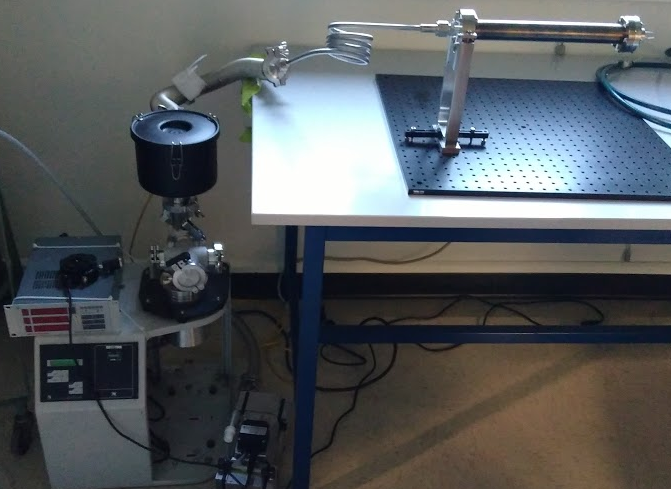
\includegraphics[width=.49\textwidth]{figs/todo/oldsetup.png}
    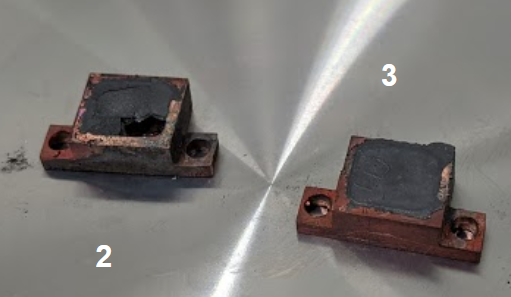
\includegraphics[width=.49\textwidth]{figs/todo/smalltarget.png}
    \caption{The `old' setup for target making and the small targets used by a
    previous beam source.}
    \label{oldsetup}
\end{figure}

The purpose of the coiled tube is to provide thermal isolation between the hot
vacuum chamber and the pumping station, as well as to make sure there is no
clear line of sight enabling the TlF molecules to make it to the vacuum pump.
The expectation is that once a TlF molecules hits a cold wall (the stainless
tube remains cold enough even while the nipple is heated up to 420\degC), it
will most likely stick there and not move further to contaminate the pump; it is
very unlikely that the TlF would survive multiple bounces. Nevertheless, the
bellows is filtered by a vacuum pump filter (A\&J Vacuum Services, part number
PN17736 or CSL-848-NW40B, rated for 99\%\ removal efficiency standard to 2
micron), which is attached to a small turbo pump. Between the filter and the
turbo, there is a Pirani gauge to measure the pressure. When the filter is new,
or if it has been open to atmosphere, it may take a long time to pump down as
water gets removed from the internal surfaces; this can be accelerated by
heating the filter to approx.\ 70\degC. Before the oven is contaminated with
TlF, it can be leak checked using an RGA or a leak checker.

Inside the nipple, on the side connected to the pump, there is a simple heat
shield (Fig.~\ref{heat_shield}) constructed of a 3" long 1/4-20 threaded rod,
which holds three stacks of five circles cut out of aluminum foil. The circles
are held in place with nuts and washers.

\begin{figure}
    \centering
    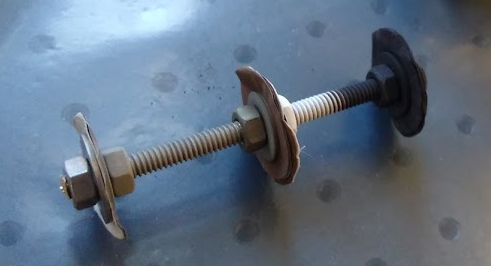
\includegraphics[width=.6\textwidth]{figs/todo/heat_shield.png}
    \caption{The heat shield inside the vacuum oven.}
    \label{heat_shield}
\end{figure}

The target holders (Fig.~\ref{oldsetup}, right) are screwed onto a copper block
using two Phillips head screws. The same block also has two tapped holes used to
attach two pairs of thermocouple wires using washers and screws; it was found
necessary to use two thermocouples since one often stopped working. The
thermocouple wires are attached to the feedthrough inside large diameter ceramic
braid, around which UHV aluminum foil is wrapped to serve as a heat shield.
Before filling the target holder with TlF powder, a copper foil is tightly
wrapped around the target holder and the copper block to create a lid. Two
additional layers of aluminum foil are wrapped around the copper foil. (Aluminum
foil must not come into direct contact with TlF; at high temperatures TlF can
react with aluminum and penetrate the lid.)

Up to this point the setup has been `clean' with not TlF present. Before the TlF
can be loaded into the oven, the nipple has to be covered by a glovebag that is
inflated using a low-pressure nitrogen line and deflated through a HEPA filter.
Before sealing the bag, make sure it contains all the necessary tools and
supplies: the thermocouple/target holder assembly, a spatula, small flat and
Phillips screwdrivers, nuts/bolts and wrench for the CF flange, new conflat
gasket, a box to contain the tools, a bottle of TlF powder, the copper and
aluminum foil lids, and alumina plate. Gloves and N95 respirators had to be worn
from the point when TlF is introduced onwards.

Working through the glovebag, the target holder, already mounted on the copper
block, is filled with the TlF powder. Once the holder is full, press down on the
powder to compact it and refill as needed, until the TlF is flush with the
surface of the holder. After wrapping the target holder and the copper block
with the copper and the two aluminum foils, the block is inserted horizontally
inside the nipple on top of an alumina plate. The alumina plate ensures uniform
heating of the copper block due to black body radiation rather than conduction
by contact with the nipple. After the assembly is inserted into the nipple, the
nipple can be closed by attaching the thermocouple feedthrough and pumps can be
started.

To remove the glovebag, the nitrogen needs to be extracted through the HEPA
filter, and then the useful tools and supplies can be removed from the glovebag
by sealing them in a part of the bag before cutting it off from the remainder of
the bag. Once the bag is removed, the nipple is cleaned with water and Kimwipes
and wrapped with heater tape. A thermocouple is secured between the nipple and
the heater tape to measure the external temperature. Finally, the heater-wrapped
chamber is wrapped with aluminum foil.

The cooling part of the procedure requires two pairs of heat resistant gloves,
such that the smaller gloves fit inside the larger gloves. We also need a wash
bottle with DI water, a box of large Kimwipes, and an assembly of three fans
Attached to a piece of wood, such that they can be moved around as a single
unit.

The heating and cooling procedure is as follows:
%
\begin{enumerate}
   \item Heat the outside of the nipple to 270\degC\ for an hour, while checking
      the temperature every ten minutes.
   \item When the inside temperature reaches 240\degC, increase the outside oven
      temperature to 425\degC\ and monitor inside temperature.
   \item When the inside temperature reaches 325\degC, turn off the heaters.
   \item When the inside temperature reaches 327\degC, remove the aluminum foil.
   \item When the inside temperature reaches 333\degC, remove the heater tape
      and start a timer.
   \item When 3 minutes are up, turn on the cooling fans and spray the outside
      of the chamber with DI water.
   \item When the outside temperature of the nipple drops below 100 degrees,
      wrap the nipple with wet Kimwipes and position the fans to blow on the wet
      Kimwipes. The internal temperature should drop to 250\degC\ within 20~min.
\end{enumerate}

After the setup has cooled down, the target is removed from the chamber and a
new target holder can be loaded to make another target. Of course, whenever the
vacuum chamber is opened, the nipple has to be enclosed in a glovebag.

\subsubsection{Adapting the setup for larger targets}

The \CENTREX\ beam source uses larger targets (Fig.~\ref{setup2}, left) than
would fit into the old target making setup. Thus I have replaced the CF2.75
nipple with a CF3.38 nipple (LDS Vacuum Products, Inc., p.n.\ 338-200-N), with
reducers (LDS Vacuum Products, Inc., p.n.\ 338x275-RN) on each side to allow it
to connect to the old VCR and thermocouple feedthroughs. The chromel/alumel
thermocouple wires (Omega HH-J-24, max.\ temp.\ 704\degC) attach to a copper
target holder cover using brass 4-40 screws. Both the new target holders and the
cover, with thermocouple wires attached, can be seen in Fig.~\ref{setup2}.

\begin{figure}[b]
    \centering
    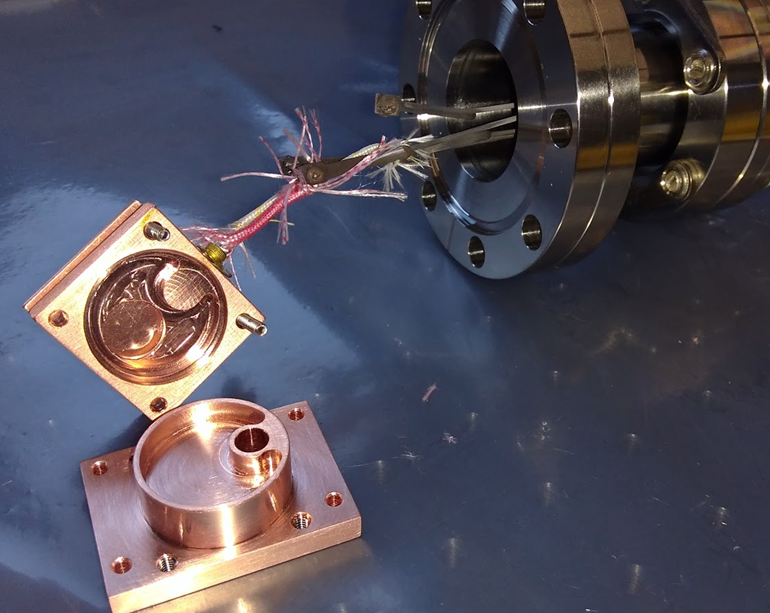
\includegraphics[height=.3\textwidth]{figs/todo/new_holder.png}
    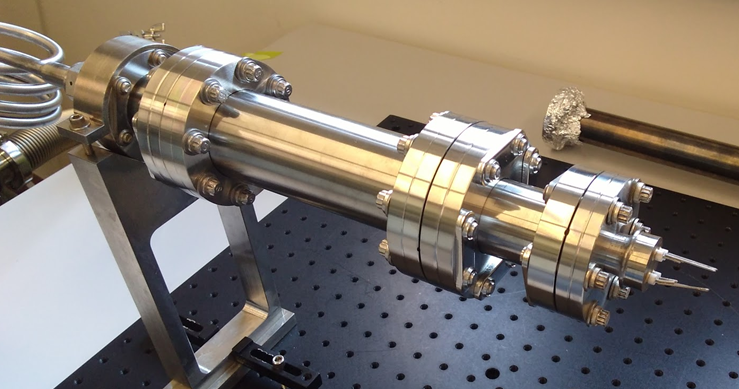
\includegraphics[height=.3\textwidth]{figs/todo/new_chamber.png}
    \caption[Target making setup adapted for new targets.]{\part{Left} New target
    holder and cover. \part{Right} Adaptation of the `old' setup to allow for
    larger target holders.}
    \label{setup2}
\end{figure}

As before, the pressure is measured by a Pirani gauge (Edwards APGX-L-NW16/ALI)
and pumped by the Leybold HY.CONE 60 turbo pump. The turbo is backed by a
diaphragm pump (Pfeiffer MVP 015-4). The nipple was wrapped with heater tape
(Omegalux STH101-040) and thermocouples read out using a readout unit (Omega
HH506R or PerfectPrime TC2100). The heating tape is powered by a model SC-10M
variac transformer. Before contaminating the setup with TlF, I have tested the
vacuum as well checked that the heating and cooling procedures are able to reach
the desired target temperature.

Dispensing with the use of the glovebag, I followed the following safety
precautions during the target making procedure: Wear gloves and a N95 respirator
mask whenever handling macroscopic (i.e., visible) amounts of TlF.  Wear gloves
whenever handling the contents of the nipple. Cover the part of the table under
the nipple with a plastic sheet.  Change gloves between handling TlF and
non-contaminated things such as the vacuum chamber wrenches and bolts. Collect
any spilled TlF inasmuch as possible.  As soon as possible, wrap the plastic
sheet up, together with contaminated gloves, used copper gasket, etc. Wrap with
packing tape, place in a ziploc bag, wrap it with packing tape, and place in
the box of TlF-contaminated waste.

\begin{figure}
    \centering
    1.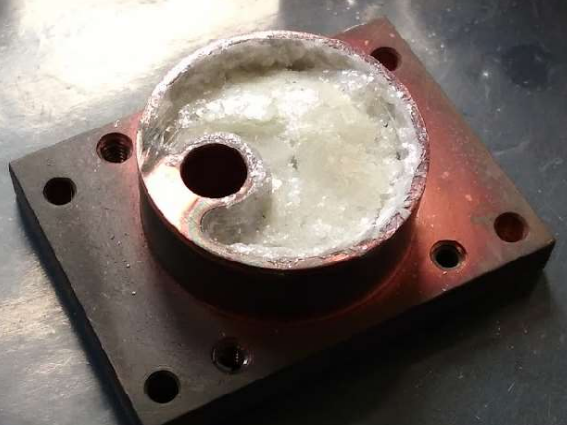
\includegraphics[height=.3\textwidth]{figs/todo/t1.png}
    \hfill
    2.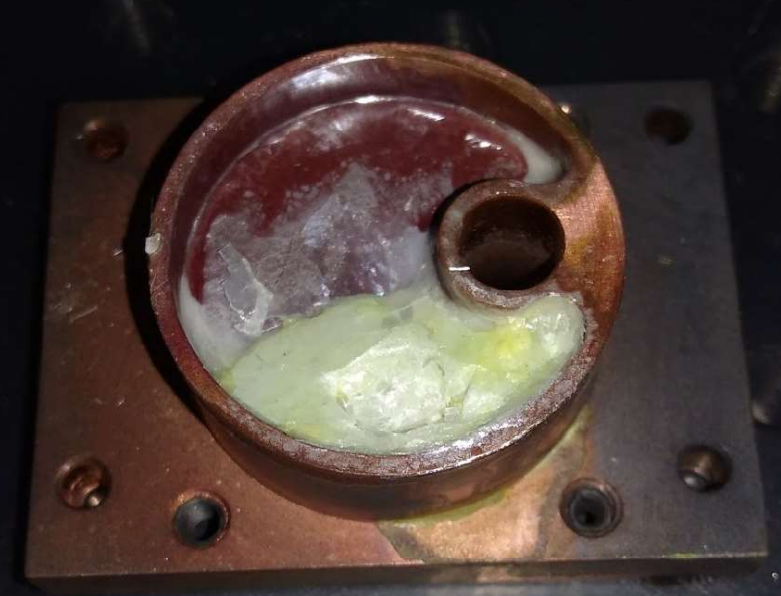
\includegraphics[height=.3\textwidth]{figs/todo/t2.png}

    \vspace{1cm}

    3.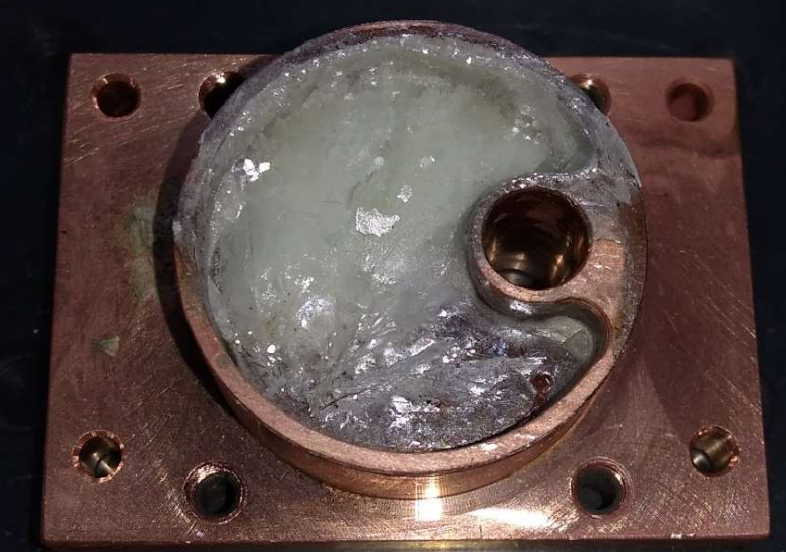
\includegraphics[height=.3\textwidth]{figs/todo/t3.png}
    \hfill
    4.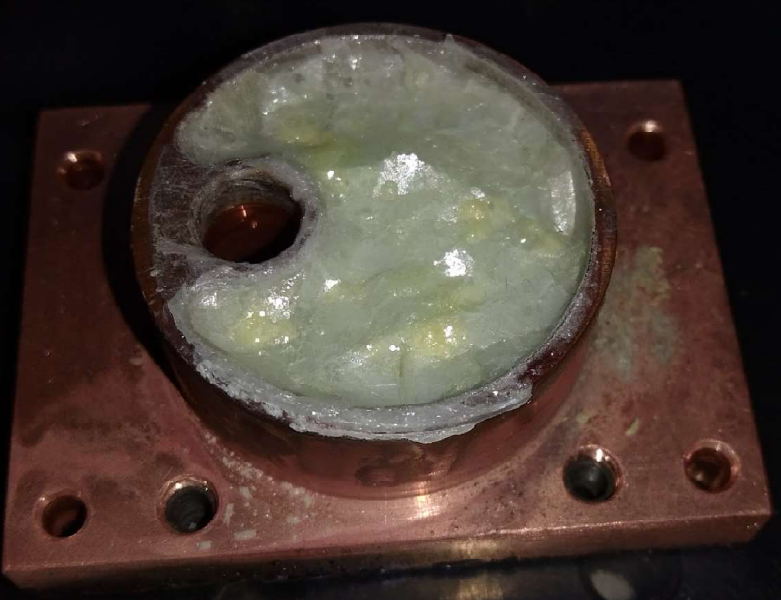
\includegraphics[height=.3\textwidth]{figs/todo/t4.png}

    \vspace{1cm}

    5.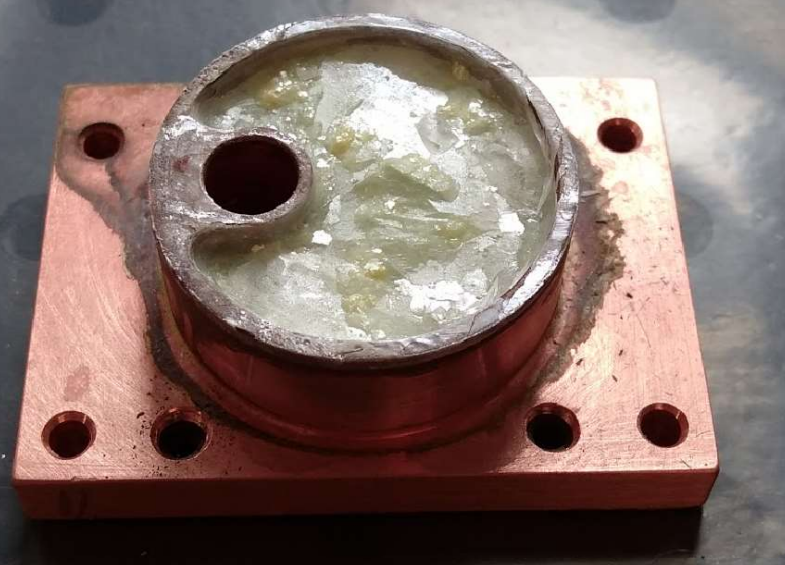
\includegraphics[height=.3\textwidth]{figs/todo/t5.png}
    \caption{First (failed) attempts at making a target.}
    \label{failed_targets}
\end{figure}

The first attempts at producing a target were not successful
(Fig.~\ref{failed_targets}). The solid surface of the TlF has a crystalline
appearance and in one case (number 2.) had a bubble, showing that the TlF was
not just molten, but boiling. I do not know why the TlF appears green after the
melting when the powdered form was white.  In each case, I was aiming to heat
the outside of the nipple enough to heat the target holder inside to a
temperature slightly above 327\degC. Even though the temperature never exceeded
337\degC, a large part of the TlF has evaporated. In one of the experiments
(number 5.), the maximum inner temperature was 322\degC\ which should not have
melted the TlF (melting point 327\degC), but it is obvious from looking at the
target that the TlF did melt. This shows that there must have been a problem
with the temperature measurement, either the sensor, the readout, or there might
have been a large temperature inhomogeneity in the setup itself.

\subsubsection{Heater inside the vacuum}

In the next version of the setup, I have attempted to improve the responsiveness
of the heating (to minimize the time spent about the melting point of TlF).
Rather than heating the outside of the nipple, the idea is to use the heater
(McMaster p.n.\ 3619K31, 120~V, 75~W) directly in the vacuum chamber
(Fig.~\ref{inside_heater}). The target holder is sandwiched between an OFHC
copper plate on top, and a stainless plate on bottom, with the heater clamped on
the copper plate. The assembly is held together with a 1/4-20 threaded rod with
wing nuts on top allowing easy disassembly (small screws have been problematic
in the past since they get filled with TlF and are thus very difficult the
turn).

\begin{figure}
    \centering
    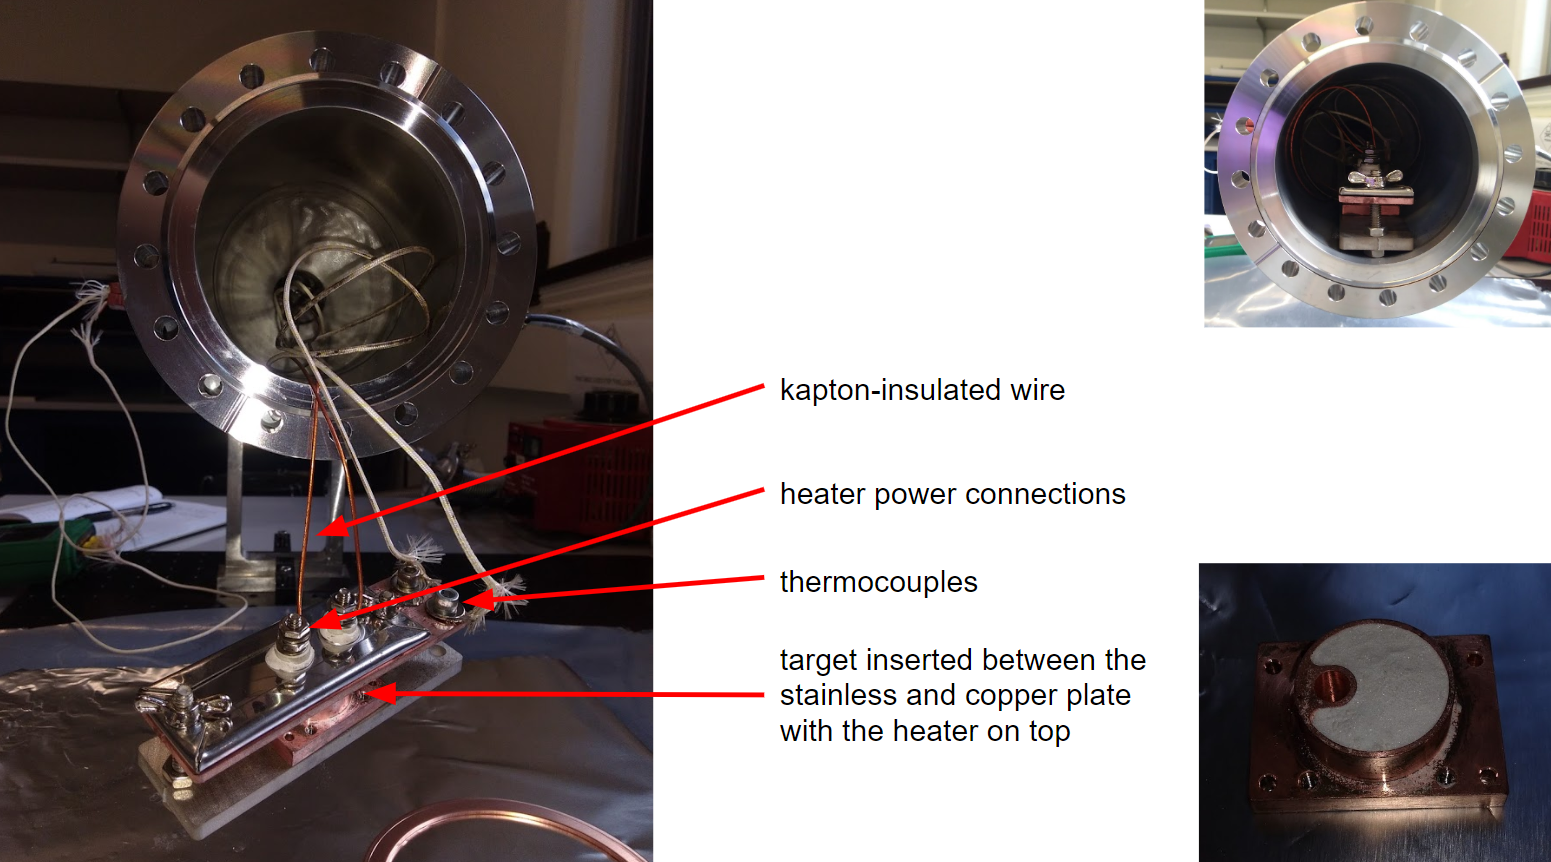
\includegraphics[width=\textwidth]{figs/todo/inside_heater.png}
    \caption{Improved target-making setup: heater located inside the vacuum chamber.}
    \label{inside_heater}
\end{figure}

The larger size of what goes inside the vacuum chamber necessitated another
nipple change, to the 6" conflat nipple used in the current setup
(Fig.~\ref{large_oven}). This setup uses a 4-way vacuum cross so that both the
electrical connections (thermocouple wires, power for the heater) and the vacuum
pump are attached to the same side of the nipple. The target holders can be
taken inside and out of the chamber by removing the CF blank on the right side
of the nipple, which simplifies the workflow.

\begin{figure}
    \centering
    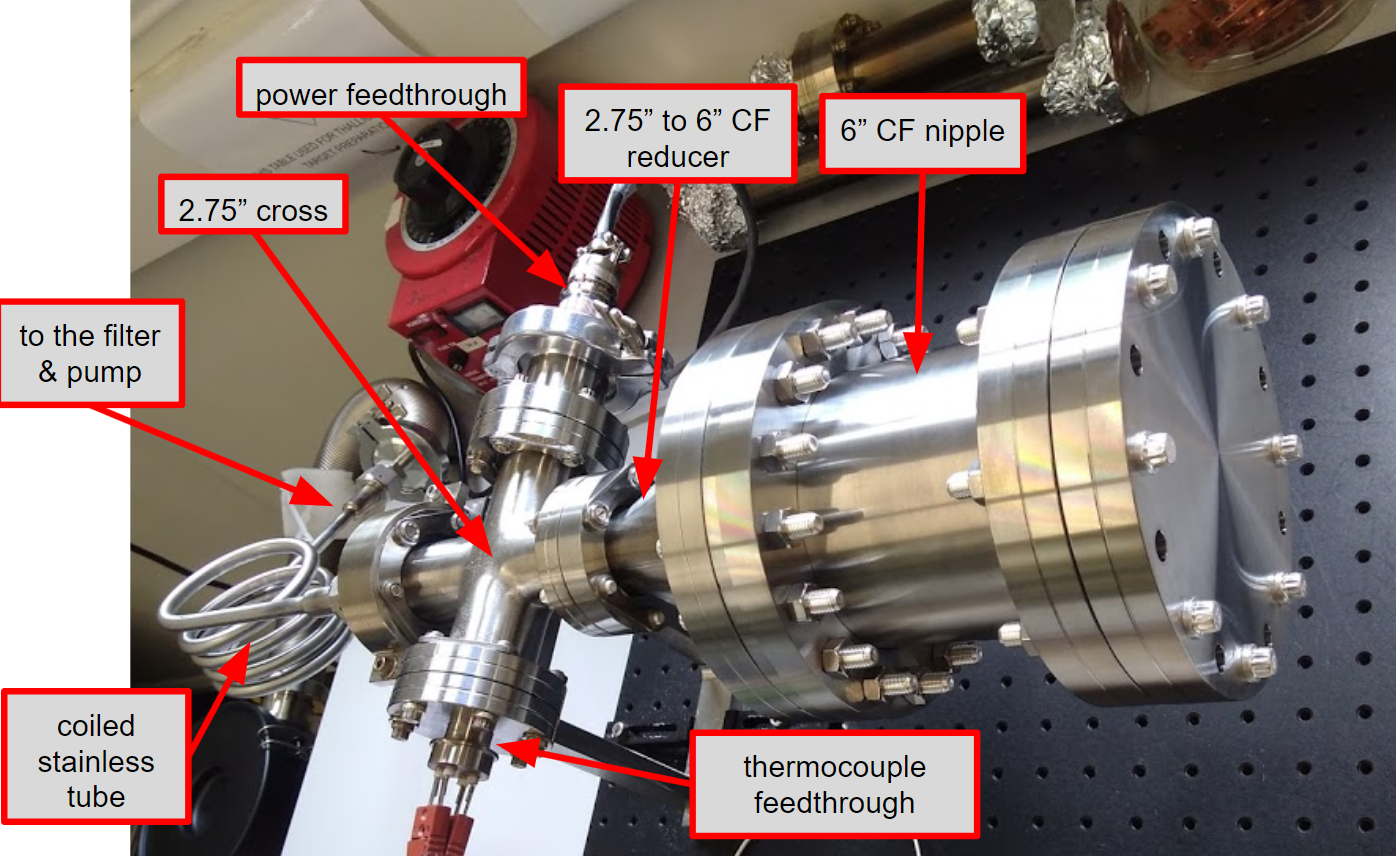
\includegraphics[width=\textwidth]{figs/todo/large_oven.png}
    \caption{The larger vacuum chamber for the heater-inside-vacuum target making
    setup, incl.\ a cross for the power feedthrough.}
    \label{large_oven}
\end{figure}

The new heater configuration again required some experimentation to find the
correct temperature profile (Fig.~\ref{making_good_target}). The difference
between not melting the TlF at all, and evaporating too much of up (which leaves
a green, crumbly, crystalline form of the TlF in the target holder) is up to the
temperature-vs-time profile of the heating. In principle, this should be easy to
reproduce by keeping the same heater power, but in practice there is a large
variation of the heat loss by conduction to the vacuum chamber either by metal
parts touching it, or via the vaporized TlF present in the chamber. In the first
two experiments shown in Fig.~\ref{making_good_target}, the heater--target
assembly was wrapped in ceramic sleeving to insulate it and allow a quick rise
in temperature above the melting point, as in the old target-making procedure.

\begin{figure}
    \centering
    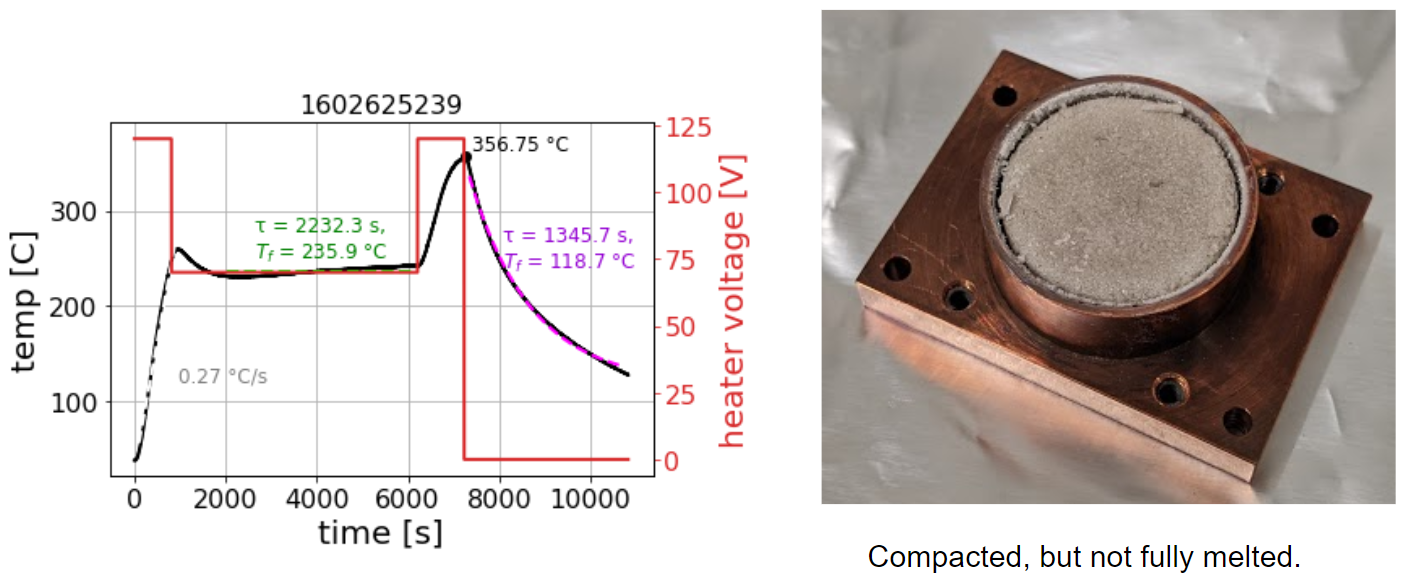
\includegraphics[width=\textwidth]{figs/todo/n1.png}
    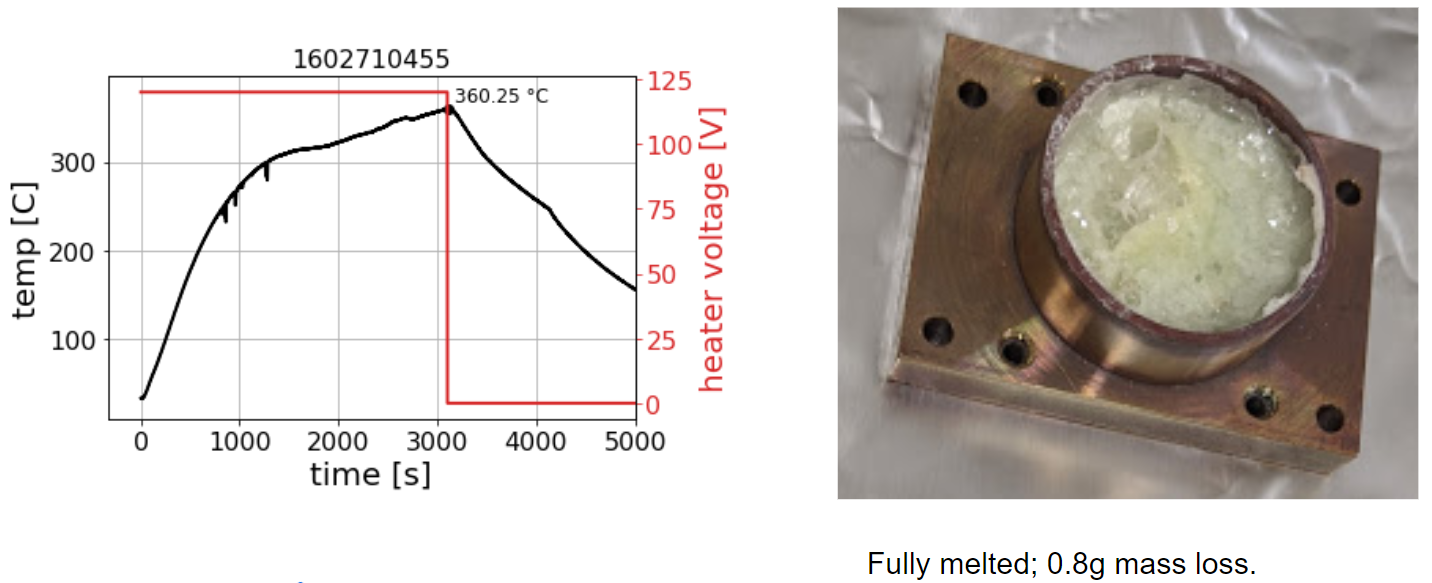
\includegraphics[width=\textwidth]{figs/todo/n3.png}
    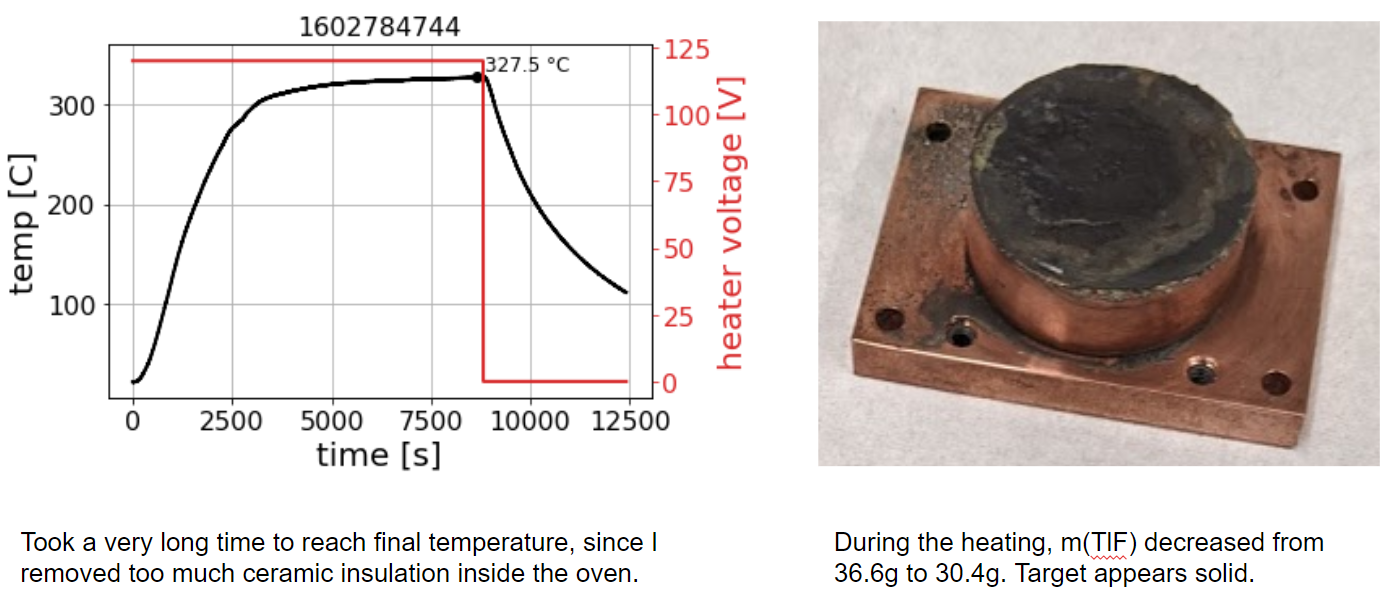
\includegraphics[width=\textwidth]{figs/todo/n4.png}
    \caption{Temperature and heater power profile and the resulting targets.}
  \label{making_good_target}
\end{figure}

When I removed ``too much'' of this insulation, the heater was barely able to
reach the melting point after a very long time (about two and a half hours!).
In principle, keeping the target so close to the melting point for such a long
time should have resulted in a large loss of TlF from the target. Instead, I was
surprised to obtain a very solid-looking target where the TlF has a glassy,
amorphous-looking surface of a dark gray color. This target has stood up well
over a long period of ablation in the cryogenic beam source.

Since producing the successful target, I have upgraded the target making system
once more (Fig.~\ref{last_oven}) in an attempt to make it even easier to use.
Now, the target holder is directly clamped onto the heater using a U-bolt. Since
the U-bolt mounting plate is made of zinc-plated steel, the target holder needs
to be covered by a copper foil to avoid unexpected chemical reactions. As shown
in Fig.~\ref{last_oven}, the thermocouple is clamped below the target holder,
but it can also be placed between the U-bolt mounting plate and the copper foil
to be more directly measuring the temperature of the TlF.

Unfortunately, I have failed to produce good targets using the new heater
arrangement. In both of the attempts shown in Fig.~\ref{last_targets}, I have
applied full heater power in order to minimize the time spent above the melting
point of TlF in accordance with the old target-making principles. The
temperature overshot in both attempts and most of the TlF was found to be
evaporated. Furthermore, due to the large amount of TlF evaporated, the inside
of the oven was covered in a very fine white `snow' of TlF dust. Part of that
was lifted by air currents upon opening the chamber, potentially contaminating
some of the work surface.

For future target making experiments, the work will need to be performed inside
a glove box (Cleatech 2300-2-A). Regardless of the heater arrangement (both the
approach in Fig.~\ref{inside_heater} and Fig.~\ref{last_oven} appear sensible),
it may be a good idea to try and reproduce the conditions that led to the good
target shown in Fig.~\ref{making_good_target}. Namely, the heater--target
assembly was placed in the vacuum chamber with minimal ceramic insulation, which
probably led to good thermal contact, which in turn facilitated fast cooling as
soon as the heater power was turned off, which presumably helped avoid an
overshoot in temperature. Furthermore, it appears that spending a long time near
the melting point is not a problem. Instead, it may be the best approach to
ensure that we reach precisely the melting point without the risk of exceeding
it too much. Of course, it is not clear how precise the temperature measurement
really is; it is possible that the temperature reached was slightly below the
melting point, allowing the TlF to fuse together in a better way than that
reached by true liquefaction.

\begin{figure}
    \centering
    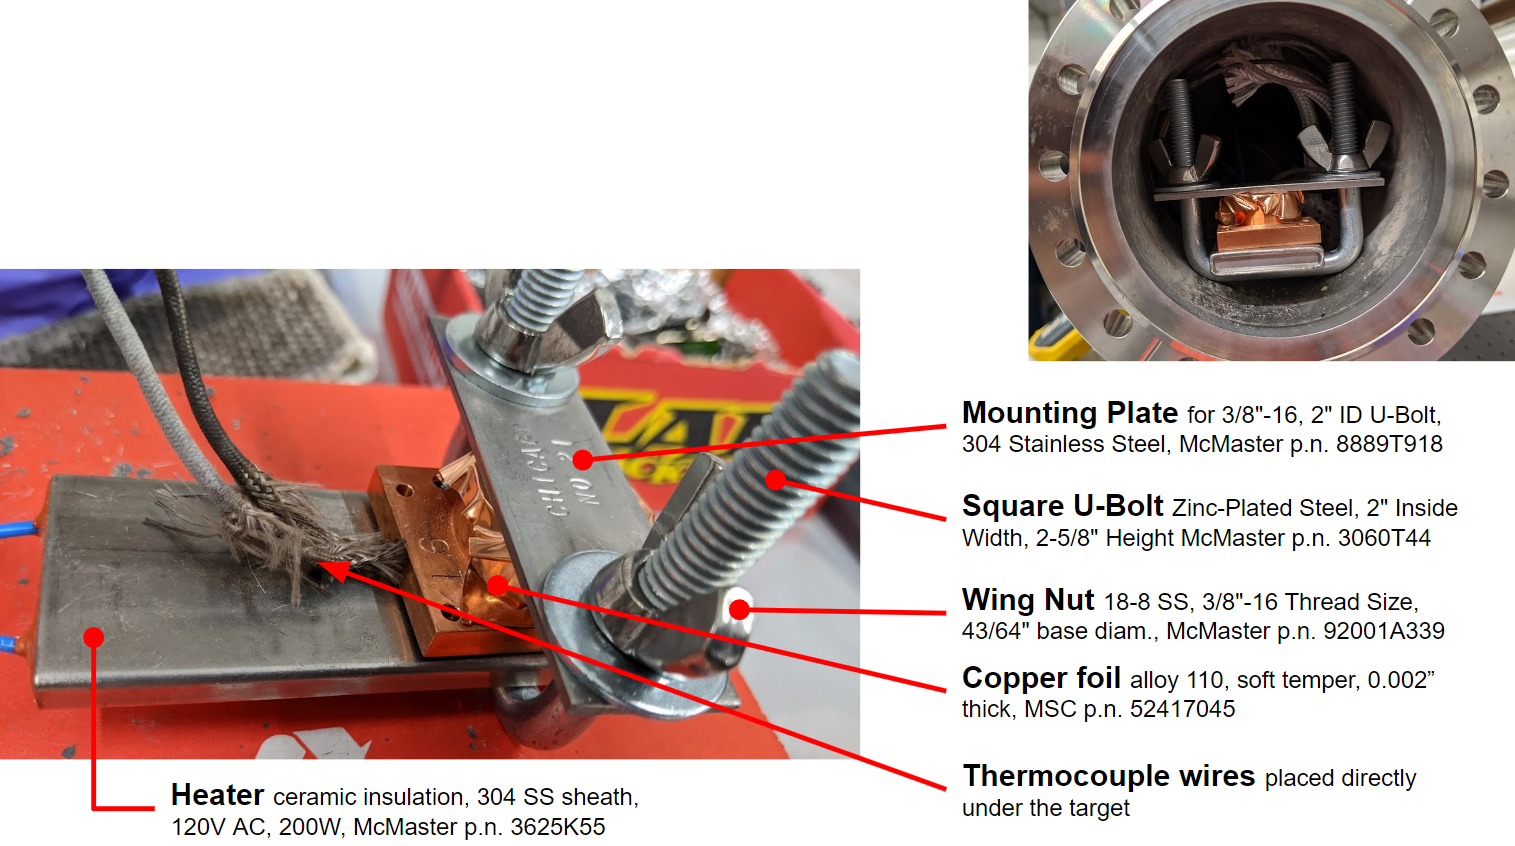
\includegraphics[width=\textwidth]{figs/todo/last_oven.png}
    \caption{New heater arrangement.}
    \label{last_oven}
\end{figure}

\begin{figure}
    \centering
    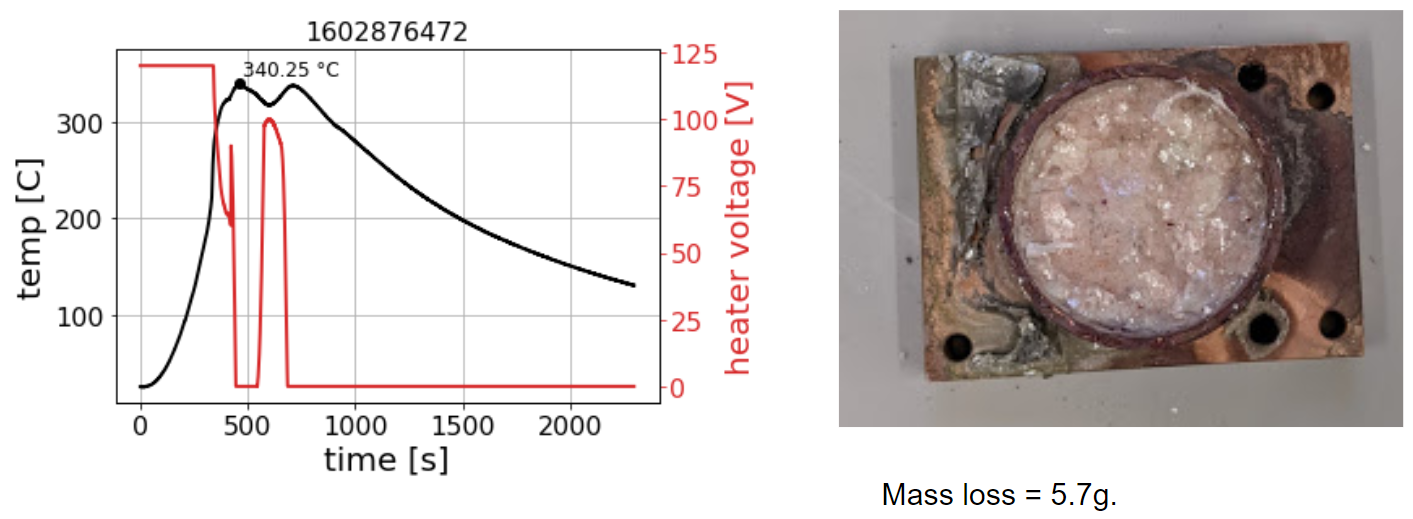
\includegraphics[width=.95\textwidth]{figs/todo/l1.png}
    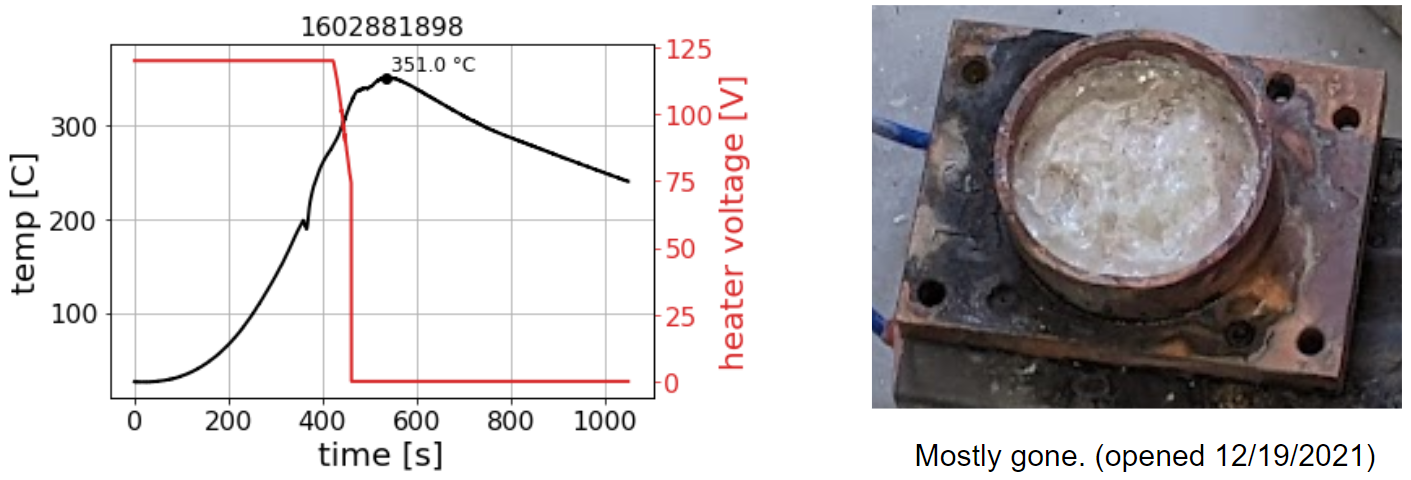
\includegraphics[width=.95\textwidth]{figs/todo/l2.png}
    \caption{Failed attempts to produce targets using the upgraded heater
    (Fig.~\ref{last_oven}).}
    \label{last_targets}
\end{figure}

\subsection{Future improvements}

\subsubsection{Temperature feed-forward}

\textit{Work reported in this subsection done together with Luke Robert Verchick
Molbak.}

Pulse tube cryocoolers operate using a process that results in periodic
(approx.\ 1.4~Hz) audible noise that is accompanied by corresponding temperature
oscillations (Fig.~\ref{T_osc}). Due to the slow response of the thermal system,
PID control is largely ineffective against these temperature variations. In this
section, we consider the feasibility of attenuating them using a feed-forward
scheme synchronized to an electronic control signal derived directly from the
compressors that power the cryocoolers.

\begin{figure}
    \centering
    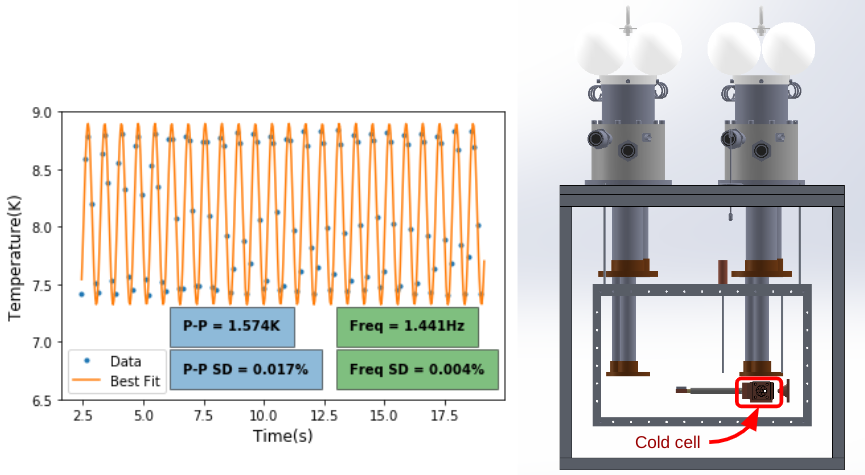
\includegraphics[width=\textwidth]{figs/todo/T_osc.png}
    \caption{Cold cell temperature oscillation inside the beam source.}
    \label{T_osc}
\end{figure}

For a general linear time-independent systems, the response $R[\delta(t)]$ of
the system to an impulse excitation $\delta(t)$ is the derivative of the
response to a step excitation $\theta(t)$:
%
\[
    R[\delta(t)]=(\d/\d t)R[\theta(t)].
\]
%
For an arbitrary control input $C(t)$, the system responds with a response that
is the convolution of the step response with the control input:
%
\[
    R[C(t)]=R[\delta(t)]\ast C(t).
\]
%
The inverse problem is to find the control $C(t)$ that is required to get a
given response $R[C(t)]$ given the step response $R[\delta(t)]$ is
(Fig.~\ref{impulse_response})
%
\[
    C(t)=\deconvolve\big(R[C(t)], R[\delta(t)]).
\]

\begin{figure}
    \centering
    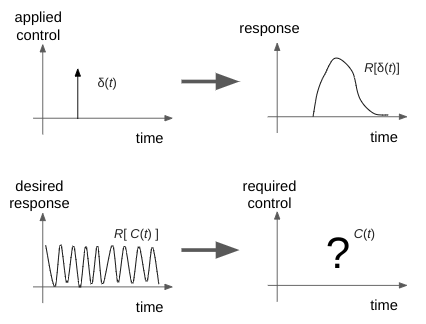
\includegraphics[width=.65\textwidth]{figs/todo/impulse_response.png}
    \caption[Impulse and response.]{Impulse and response. \part{Top} Applying an
    impulse $\delta(t)$ to the input of a control system produces an impulse
    response $R[\delta(t)]$. \part{Bottom} If we want to induce a response
    $R[C(t)]$, then we have to find the correct control $C(t)$ to apply.}
    \label{impulse_response}
\end{figure}

In this framework, we can consider the beam source to be such a control system.
The input is the heater power, $P(t)$ and the output is the cell temperature
$T(t)$. We would like to find the $P(t)$ that produces a temperature response
that best cancels out the pulse tube temperature oscillations. In principle, we
could find the step response, differentiate it to find the impulse response, and
then deconvolve it with the desire temperature profile to find the appropriate
heater power to apply. In practice, we were only able to begin work on this
before terminating the project because of external time constraints.

The feed-forward scheme would be synchronized to the pulse tube compressor
pressure variations. In order to do that, we connected a cable to the inside of
the compressor to one of the internal pressure gauges
(Fig.~\ref{compressor_signal}). We used an Arduino to filter the signal and
output a square wave synchronised to it. In the future, this signal can be used
to drive a heater in sync with it in the hope of thereby minimizing the cell
temperature oscillations.

\begin{figure}
    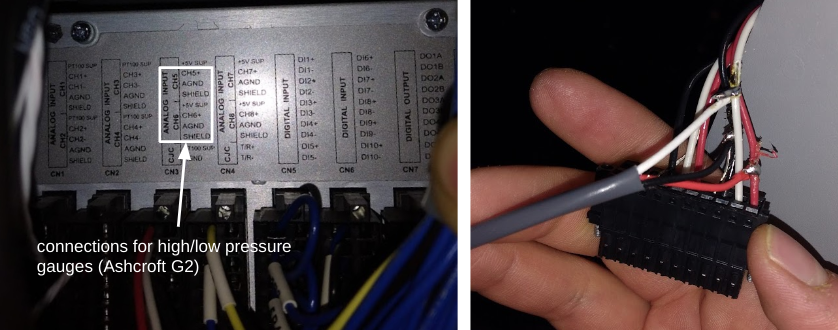
\includegraphics[width=.66\textwidth]{figs/todo/compressor_conn.png}
    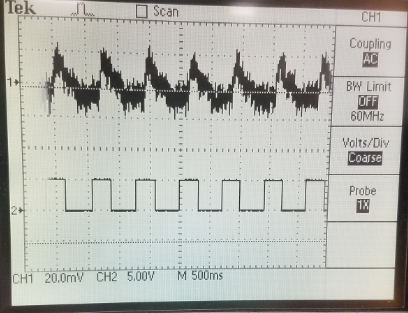
\includegraphics[width=.33\textwidth]{figs/todo/filtered_signal.png}
    \caption[Pulse tube sync signal.]{\part{Top} Pulse tube sync signal
    extraction. \part{Left} The connection for high and low pressure pressure
    gauges inside the compressor. \part{Middle} A cable can be soldered to one
    of the pressure gauge connectors to extract the signal. \part{Right} The
    extracted signal. The upper trace is the original signal from the
    compressor, while the lower trace is the Arduino output after filtering the
    original signal and syncing that signal to the Arduino.}
    \label{compressor_signal}
\end{figure}

\subsubsection{Continuous beam source}

The beam source as described above is ablated using a pulsed laser, therefore
the beam source itself is pulsed. However, laser ablation is not the only method
to load the cell of a cryogenic beam source with the species of interest. Other
demonstrated methods include cell loading from a molecular beam, cryogenic
discharge \cite{doyle1995buffer}, direct gas flow, and capillary fill. In the
latter method, a thin hot tube is inserted into the cell (Fig.~\ref{capillary}).
Despite the lack of direct thermal contact between the capillary and the cell,
this method is limited to molecules that vaporize at a low enough temperature
such that the cell and the buffer gas inside it are not subject to more
heating (through radiation and gas conduction) than can be offset by the cooling
of the cell.

\begin{figure}
   \centering
    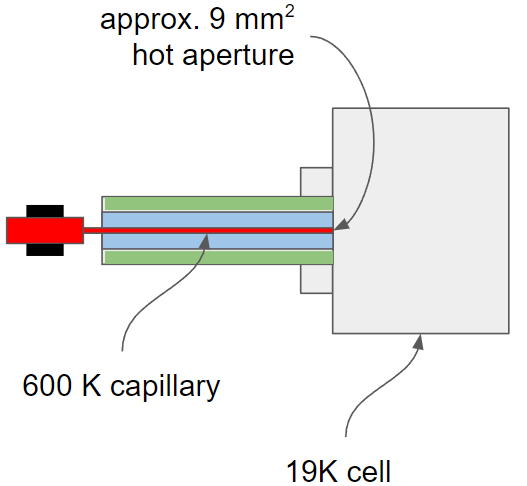
\includegraphics[width=.4\textwidth]{figs/todo/capillary.png}
    \caption{Continuous beam source: capillary fill.}
    \label{capillary}
\end{figure}

A fundamental limit is posed by the heat load delivered by the species of
interest itself, assuming no additional heat load from the capillary. In the
case, we can estimate that an unacceptable amount of heating results if
\cite[eqn~4.2]{patterson2010thesis}
%
\[
   {\phi_\text{A}}>{\phi_\text{B}}\frac{T_\text{B}}{T_\text{A}},
\]
%
where the subscripts A and B refer to the species and the buffer gas,
respectively. For a typical neon flux of $\phi_\text{B}\approx40$~sccm at a
temperature $T_\text{B}\approx10$~K, the flux of hot TlF
($\phi_\text{A}\approx600$~K) would be limited to
$\phi_\text{A}\approx0.7$~sccm, or approx.\ $3\cdot10^{17}$ molecules per
second.

Let us estimate the expected flow rate through a capillary, assuming laminar
flow. According to Poiseuille's formula, the mass flow rate for a fluid of
dynamic viscosity $\mu$ through a pipe of radius $R$ and length $l$ at a
pressure drop of $\Delta p$ is \cite[eqn~17.10]{landau2013fluid}
%
\[
   Q=\frac{\pi\Delta p}{8\mu l}R^4.
\]
%
The dynamic viscosity is approximately $\mu\sim m\bar{v}N\lambda$
\cite[eqn~8.11]{pitaevskii2012physical}, where
$m=223.4\;\text{u}=2.71\cdot10^{25}$~kg is the mass of a TlF molecule
\cite{linstrom2001nist}, $\bar{v}\sim\sqrt{\kB T/m}$ is the average molecular
velocity, $N$ is the number of molecules per unit volume, and $\lambda$ is the
mean free path. At the temperature $T\approx600$~K, TlF oven pressure of
$\Delta p\approx1$~torr, and assuming a mean free path of $\lambda\sim1$~mm, we
would get a flow of approx.\ $10^{18}$ molecules per second through a $R=1/16$"
pipe of length $l=1$".

The radiative heat load from the tip of the hot capillary can be estimated to be
$\sigma T^4A=\sigma(600~\text{K})^4(3~\text{mm})^2\approx0.07~\text{W}$, which
can easily be removed by the cryocoolers. Potentially more problematic is the
heat $P_\text{Ne}$ imparted to the neon buffer gas:
%
\[
   P_\text{Ne}\sim
   \underbrace{(\pi\cdot3~\text{mm})^2}_\text{aperture area}
   \cdot
   \underbrace{\sqrt{\frac{\kB(19~\text{K})}{m_\text{Ne}}}}_\text{neon velocity}
   \cdot
   \underbrace{\frac{10^{16}}{(25~\text{mm})^3}}_\text{neon density}
   \cdot
   \underbrace{\kB(600~\text{k})}_{\substack{\text{energy imparted}\\\text{to neon on
   collision}}}
   \sim1~\text{mW},
\]
%
because it causes a buffer-gas temperature increase of
%
\[
   \Delta
   T_\text{Ne}\sim\frac{1~\text{mW}}{40~\text{sccm}\frac32\kB}=2.7~\text{K}.
\]

In the above calculation, we have assumed that there is approx.\ 1~torr of
pressure in the oven where TlF is converted into its gaseous form. In general,
the vapor (or sublimation) pressure, i.e.\ the pressure when the rate of
sublimation equals the rate of deposition of its vapor phase, is temperature
dependent. In thallium fluoride, this pressure is given by
\cite{keneshea1965thermodynamics}
%
\[
   \log\frac{p}{1~\text{torr}}=\left[-\frac{5450~\text{K}}{T}+7.841\right]\pm0.016.
\]
%
Some useful pressures are: $p(616~\text{K})\approx0.1~\text{torr}$ and
$p(695~\text{K})\approx1~\text{torr}$.

To go beyond the back-of-the-envelope estimates considered so far, it would be
useful to do simulations of the beam properties as it emerges from a buffer gas
cell. In order to know what kind of simulations would be appropriate, we can
consider the Knudsen number $\text{Kn}=\lambda/L$, where $L$ is a typical length
scale of the capillary or the cell. Given the molecular densities expected, we
operate around $0.1<\text{Kn}<10$, which is in the transition regime between
continuous and free molecular flow. \cite{shen2018multiparameter}

In this regime, Direct simulation Monte Carlo (DSMC) is an efficient method to
simulate flows. \cite{oran1998direct,birdmolecular} The method begins by
selecting a large number ($10^6$ to $10^{11}$) of ``statistically representative
particles'', each representing a number of physical particles. We also select a
time step that is less than the mean collision time and split the geometry into
a mesh of cells (smaller than the mean free path). The main algorithm loop
proceeds as follows:
%
\begin{enumerate}
   \item Move the particles given their positions and velocities.
   \item Simulate collisions between molecules and walls.
   \item Simulate collisions between randomly selected pairs of molecules within each cell.
\end{enumerate}
%
There is a number of DSMC codes available. The qualitative simulation of the
beam emerging from a 2D axisymmetric model of a cell shown in Fig.~\ref{DS2V}
was created using DS2V \cite{bird2005ds2v}. Further work could use DS2V, or a
number of other similar codes, such as SPARTA \cite{plimpton2019direct}, to
quantitatively evaluate the beam properties as a function of the injected TlF
gas flow rate, temperature, buffer gas flow rate and temperature, size and
thickness of the cell exit hole, the effect of a shaped nozzle, etc.

\begin{figure}
   \centering
    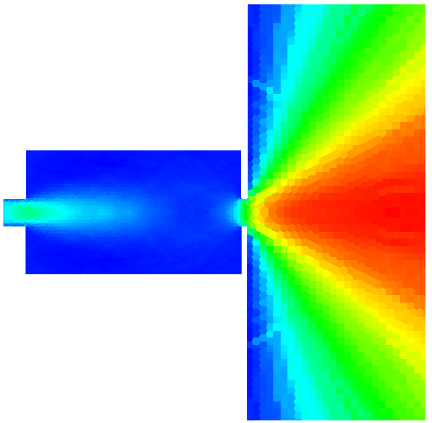
\includegraphics[width=.6\textwidth]{figs/todo/DS2V.png}
    \caption[DS2V simulation of a buffer gas cell.]{DS2V simulation of a buffer
    gas cell (qualitative depiction). Color shows velocity component along the
    beam direction (red is faster than blue).}
    \label{DS2V}
\end{figure}
